\documentclass[10pt, xcolor={dvipsnames}]{beamer}
\mode<presentation>{
  \usetheme{Madrid}
  % or ...
  %\usecolortheme[named=OliveGreen]{structure}
  \setbeamercovered{transparent}
  % or whatever (possibly just delete it)
}
\graphicspath{{../images/}}
\usepackage[utf8x]{inputenc}
\usepackage[russian]{babel}
\usepackage[usenames,dvipsnames]{pstricks}
\usepackage{epsfig}
\begin{document}
\small
\begin{frame}{Триангуляция Делоне, Триангуляция -> Граф}
\begin{itemize}
\item Берется структура в PDB.
\item Центры атомов рассматриваются как точки. По ним строится триангуляция Делоне (с помощью scipy.delaunay - обертки над алгоритмом qhull).
\item Берется невзвешенная триангуляция -- по тем же соображениям, по которым она используется в CAVER (эвристика).
\end{itemize}
Я сопоставляю графу триангуляцию по тому же принципу, как в статье по CAVER:
\begin{columns}
\begin{column}{0.5\textwidth}
\begin{center}
\resizebox{!}{0.3\textheight}{
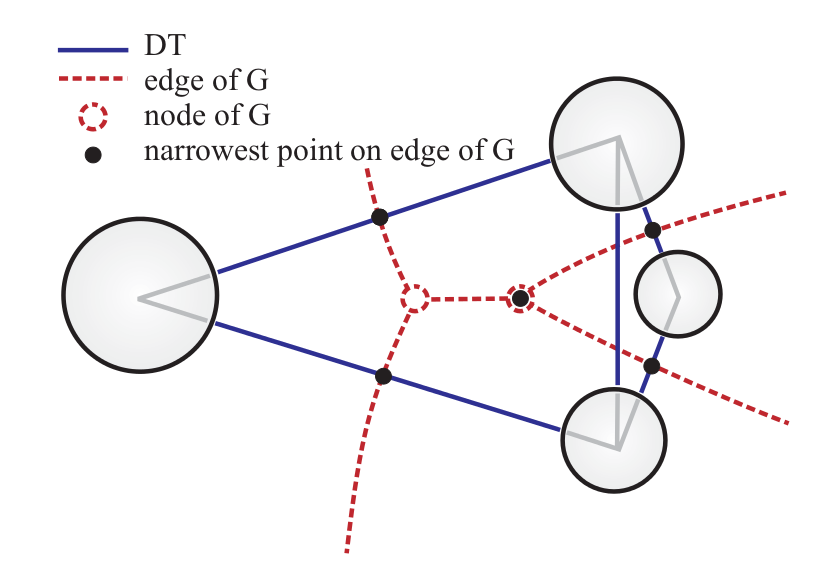
\includegraphics{algorithm/image4_caver.png}
}

[Computation of tunnels in protein molecules using
Delaunay triangulation, P.Medek, et al., 2007]
\end{center}
\end{column}
\begin{column}{0.5\textwidth}
Треугольники триангуляции -- вершины графа, ребра графа -- общие стороны треугольников (с ограничением снизу на длину).

Дополнительно используется такой же граф по треугольникам выпуклой оболочки (без ограничения снизу на длину стороны, просто по смежным по стороне треугольникам).
\end{column}
\end{columns}


\end{frame}

\begin{frame}{Алгоритм}{выбор начального множества треугольников выпуклой оболочки}
Выбирается начальное множество треугольников выпуклой оболочки. Сейчас берутся треугольники, вершины которых недалеко (в смысле отсечки по расстоянию) от второго белка.

\begin{itemize}
\item В CAVER используется алгоритм Дейкстры для поиска каналов максимальной ширины. Каналы как правило сквозные, в нашем случае это не обязательно.
\item Нам надо получить внешнюю поверхность белка, то есть все, что расположено близко к интерфейсу взаимодействия, и при этом может быть, например, карманом (углублением в поверхности) или каналом (сквозной дырой в поверхности).
\end{itemize}
\end{frame}

\begin{frame}{Поиск карманов (неудачная попытка) }
\begin{itemize}
\item Попробуем искать карманы. Для этого используем поиск в ширину с ограничением на проходимость ребер. 
\item В результате выделяются много-много атомов по всей внешней поверхности белка:
\end{itemize}
\begin{center}
\resizebox{!}{0.5\textheight}{
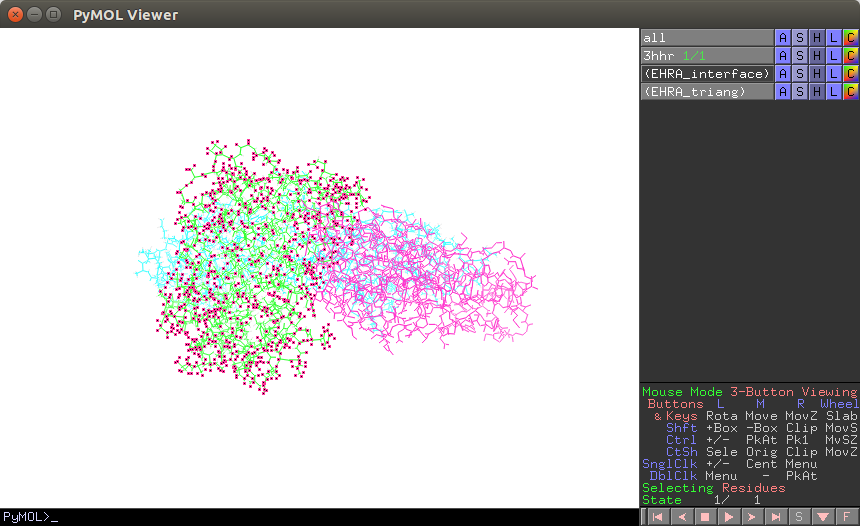
\includegraphics{algorithm/dijkstra1.png}
}
\end{center}
\end{frame}
\begin{frame}{Поиск карманов (НЕ алгоритм Дейкстры)}{как считается сейчас}
\begin{columns}
\begin{column}{0.1\textwidth}
%\begin{center}
%\resizebox{!}{0.2\textheight}{
%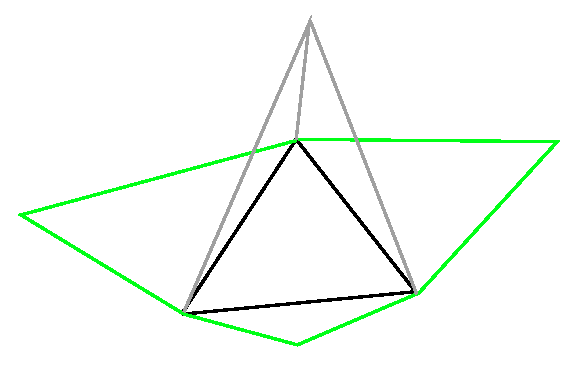
\includegraphics{triangles.eps}
%}
%\end{center}
\end{column}
\begin{column}{0.9\textwidth}
\small{
Пока все очень просто, Дейкстры близко нет:
\begin{itemize}
\item Начинаем с множества отобранных треугольников выпуклой оболочки (черным цветом)
\item Ищем в ширину с ограничениями
\item Ходим только по тем треугольникам, для которых ближайший треугольник выпуклой оболочки -- один из отобранных треугольников выпуклой оболочки, а не какой-либо из других треугольников выпуклой оболочки.
\item Ближайший треугольник == в смысле расстояния до ближайшей из вершин он ближе, чем другие треугольники выпуклой оболочки

\item (Нашла несколько статей по поиску карманов, вероятно, переделаю) 
\end{itemize}
}
\end{column}
\end{columns}


\textbf{Почему не использую Дейкстру}: не придумала, как корректно задавать порядок выбора вершин на очередном шаге для выбора нового треугольника-вершины (легко находятся контрпримеры -- я хотела нарисовать картинок сюда, но не придумала, как).
\end{frame}

\begin{frame}{Поиск карманов (что находится) }
\begin{itemize}
\item На скриншоте - темно-синим и голубым нарисованы две цепочки, на голубой выделены фиолетовым фрагменты, которые нашлись при поиске карманов указанным выше способом.
\item Фиолетовые фрагменты слева внизу - с точки зрения алгоритма корректны, они попали за счет выбора начального множества треугольников выпуклой оболочки (достаточно, чтобы одна из вершин треугольника была вблизи интерфейса взаимодействия - в этом случае именно так и получилось)
\end{itemize}
\begin{center}
\resizebox{!}{0.7\textheight}{
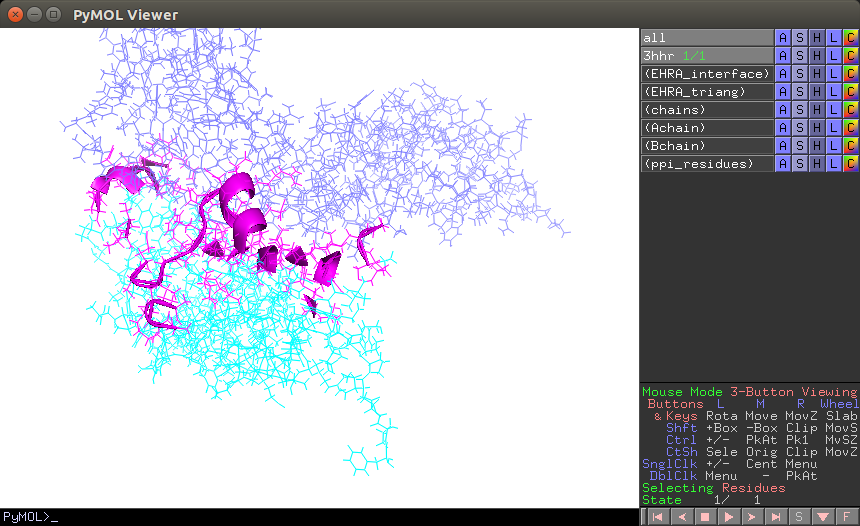
\includegraphics{algorithm/image_step2.png}
}
\end{center}
\end{frame}
\section{Петли}
\begin{frame}{Петли 0}{пояснение к скриншотам}
\begin{itemize}
\item Сейчас вторичная структура определяются на основе вывода DSSP (biopython же).

\item Я беру непрерывные фрагменты структуры, которые не определяются как альфа-спирали или бета-листы, выбираю среди них те, в которые попадает какая-либо аминокислота, ну и добавляю их к выделяемому контуру - технической сложности никакой. Содержательности - тоже :(

\item Далее несколько скриншотов с L и H цепями антитела (2OSL.pdb, но без воды) с разных ракурсов.

\item желтым цветом - L-цепь, на ней голубым выделены аминокислоты, содержащие атомы, которые попали в начальное отобранное множество треугольников выпуклой оболочки

\item Синим - то, что выделилось в результате поиска карманов

\item Красным - фрагменты цепи, которые были добавлены в результате добавления петель

\end{itemize}
\end{frame}
\begin{frame}{Петли 1}
Здесь все почти хорошо, но смущает сине-желтый кусок - но это надо поиск карманов смотреть и переделывать. И еще \textbf{сильно смущает} петля прямо по центру - у нее синие края справа и слева, при этом посередине она желтая
\begin{center}
\resizebox{!}{0.7\textheight}{
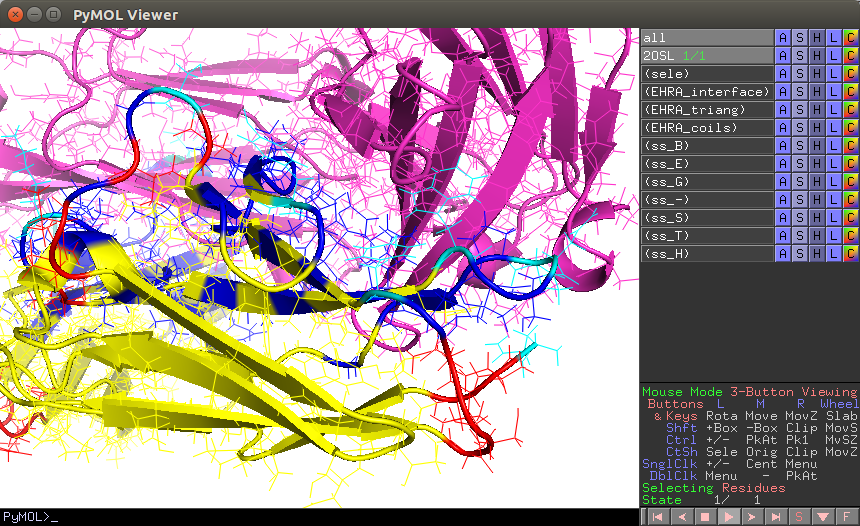
\includegraphics{algorithm/loops1.png}
}
\end{center}

\end{frame}

\begin{frame}{Петли 2}
Здесь вроде бы все хорошо (кроме сине-желтого).
\begin{center}
\resizebox{!}{0.7\textheight}{
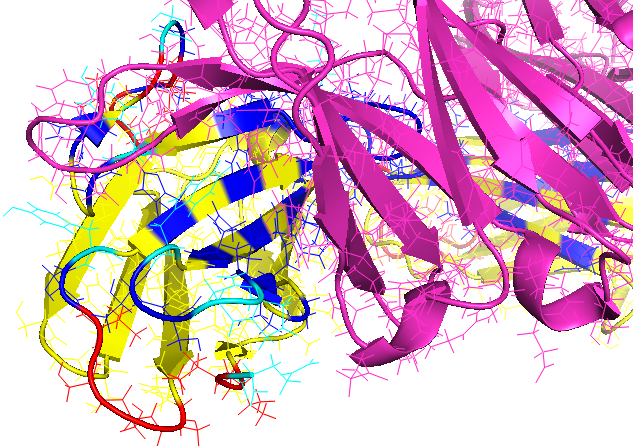
\includegraphics{algorithm/loops2.png}
}
\end{center}

\end{frame}

\begin{frame}{Петли 3}
Здесь снизу явно попала петля, которая удалена от интерфейса взаимодействия, но при этом один из атомов ее аминокислот по удачному стечению обстоятельств попал в множество отобранных треугольников выпуклой оболочки, за счет чего петля попала целиком.

Над этой петлей есть петля, которая вроде бы не влияет вообще. 

И это наводит на мысль о том, что изначальный выбор аминокислот не так хорош. Возможно, стоит использовать граф Габриэля? 
\begin{center}
\resizebox{!}{0.6\textheight}{
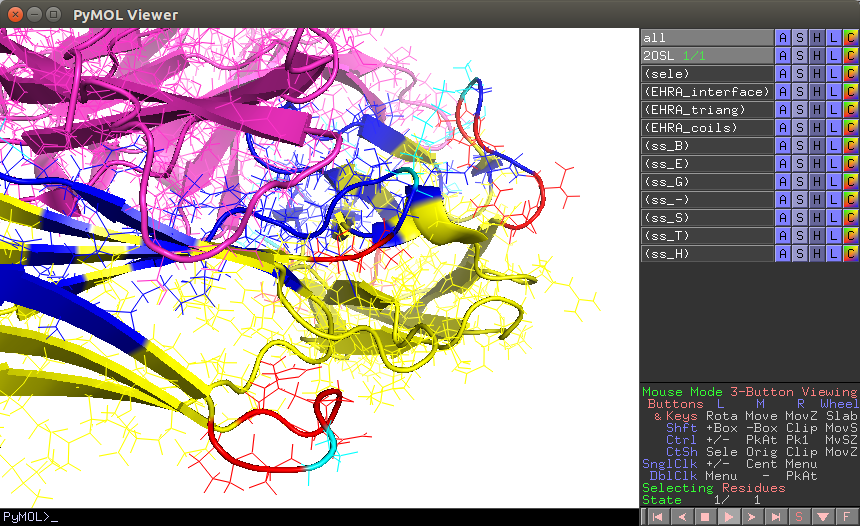
\includegraphics{algorithm/loops3.png}
}
\end{center}

\end{frame}

\begin{frame}{Петли 4}
Посередине петля полностью желтая - но это из-за способа, которым добавлялись карманы.
\begin{center}
\resizebox{!}{0.6\textheight}{
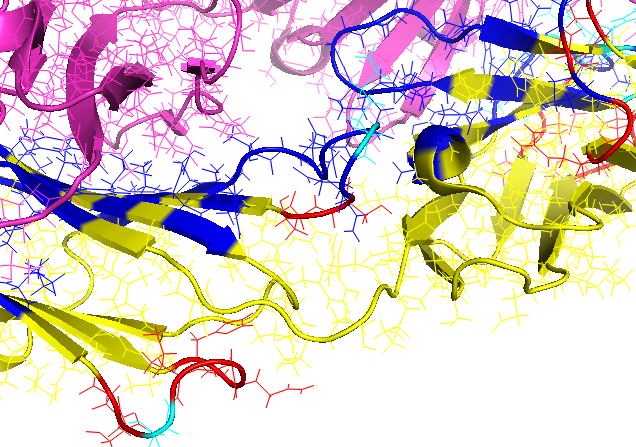
\includegraphics{algorithm/loops4.png}
}
\end{center}

\end{frame}

\begin{frame}{Идеи}
\begin{itemize}
\item Я отправляла статью про петли. Что там происходит: взята ASEdb, рассмотрены короткие фрагменты петель, содержащие энергетически горячие аминокислоты и приведена их какая-то классификация.

вариантов 2: либо не добавлять петли целиком, вместо этого добавлять только такие фрагменты (в статье они приведены), либо как-то их отмечать на выделенных петлях + отмечать на удаленных петлях, которые в выделенный регион не попали.

\item про hmm думаю, напишу через пару дней.

\item вообще если получится, я разберусь как считать взвешенную триангуляцию Делоне и с помощью нее искать карманы.

\item Еще хочу почитать про O-кольца.

\end{itemize}
\end{frame}
\end{document}